\documentclass[10pt,two column,a4paper]{article}
\usepackage[utf8]{inputenc}
\usepackage[T1]{fontenc}
\usepackage[portuguese]{babel}
\usepackage{amsmath}
\usepackage{amsfonts}
\usepackage{amssymb}
\usepackage{makeidx}
\usepackage{graphicx}
\usepackage{tikz}
\usepackage{float}
\usepackage{breqn}
\usepackage{pgfplots}
\usepackage[left=10.00mm, right=10.00mm, top=2.00cm]{geometry}
\usepackage[colorinlistoftodos,prependcaption,textsize=large]{todonotes}
\author{Victor Medeiros}
\title{Trabalho de Sistemas de Comunicações II}
\begin{document}
	\maketitle
	\section{Exercício 1}
	\todo[inline]{Plote um gráfico da probabilidade de erro de símbolo ($P_e$) em função da razão sinal-ruído por bit ($E_b/N_0$), em dB, para as modulações a seguir e analise os resultados:}
	\begin{enumerate}
	\item[a$)$] M-PAM para M = 2,4,8,16
	\item[b$)$] M-QAM para M = 4,16,64,256
	\item[c$)$] M-PSK para M = 8,16,32,64
	\item[d$)$] M-FSK para M = 2,4,8,16,32,64,128,256\end{enumerate}	
	\subsection{Modulação M-PAM}
	Foi utilizada a Equação \eqref{pam} para calcular a SER desta modulação. Com isso, foram plotadas as curvas encontradas em Figura \ref{pamI}.
	\begin{equation}
	P_e  = 2\frac{(M-1)}{2M}erfc\left( \sqrt{ \frac{3\log_2(M)SNR}{(M^2-1)} }\right)\label{pam}
	\end{equation}
	\begin{figure}[h]\centering
		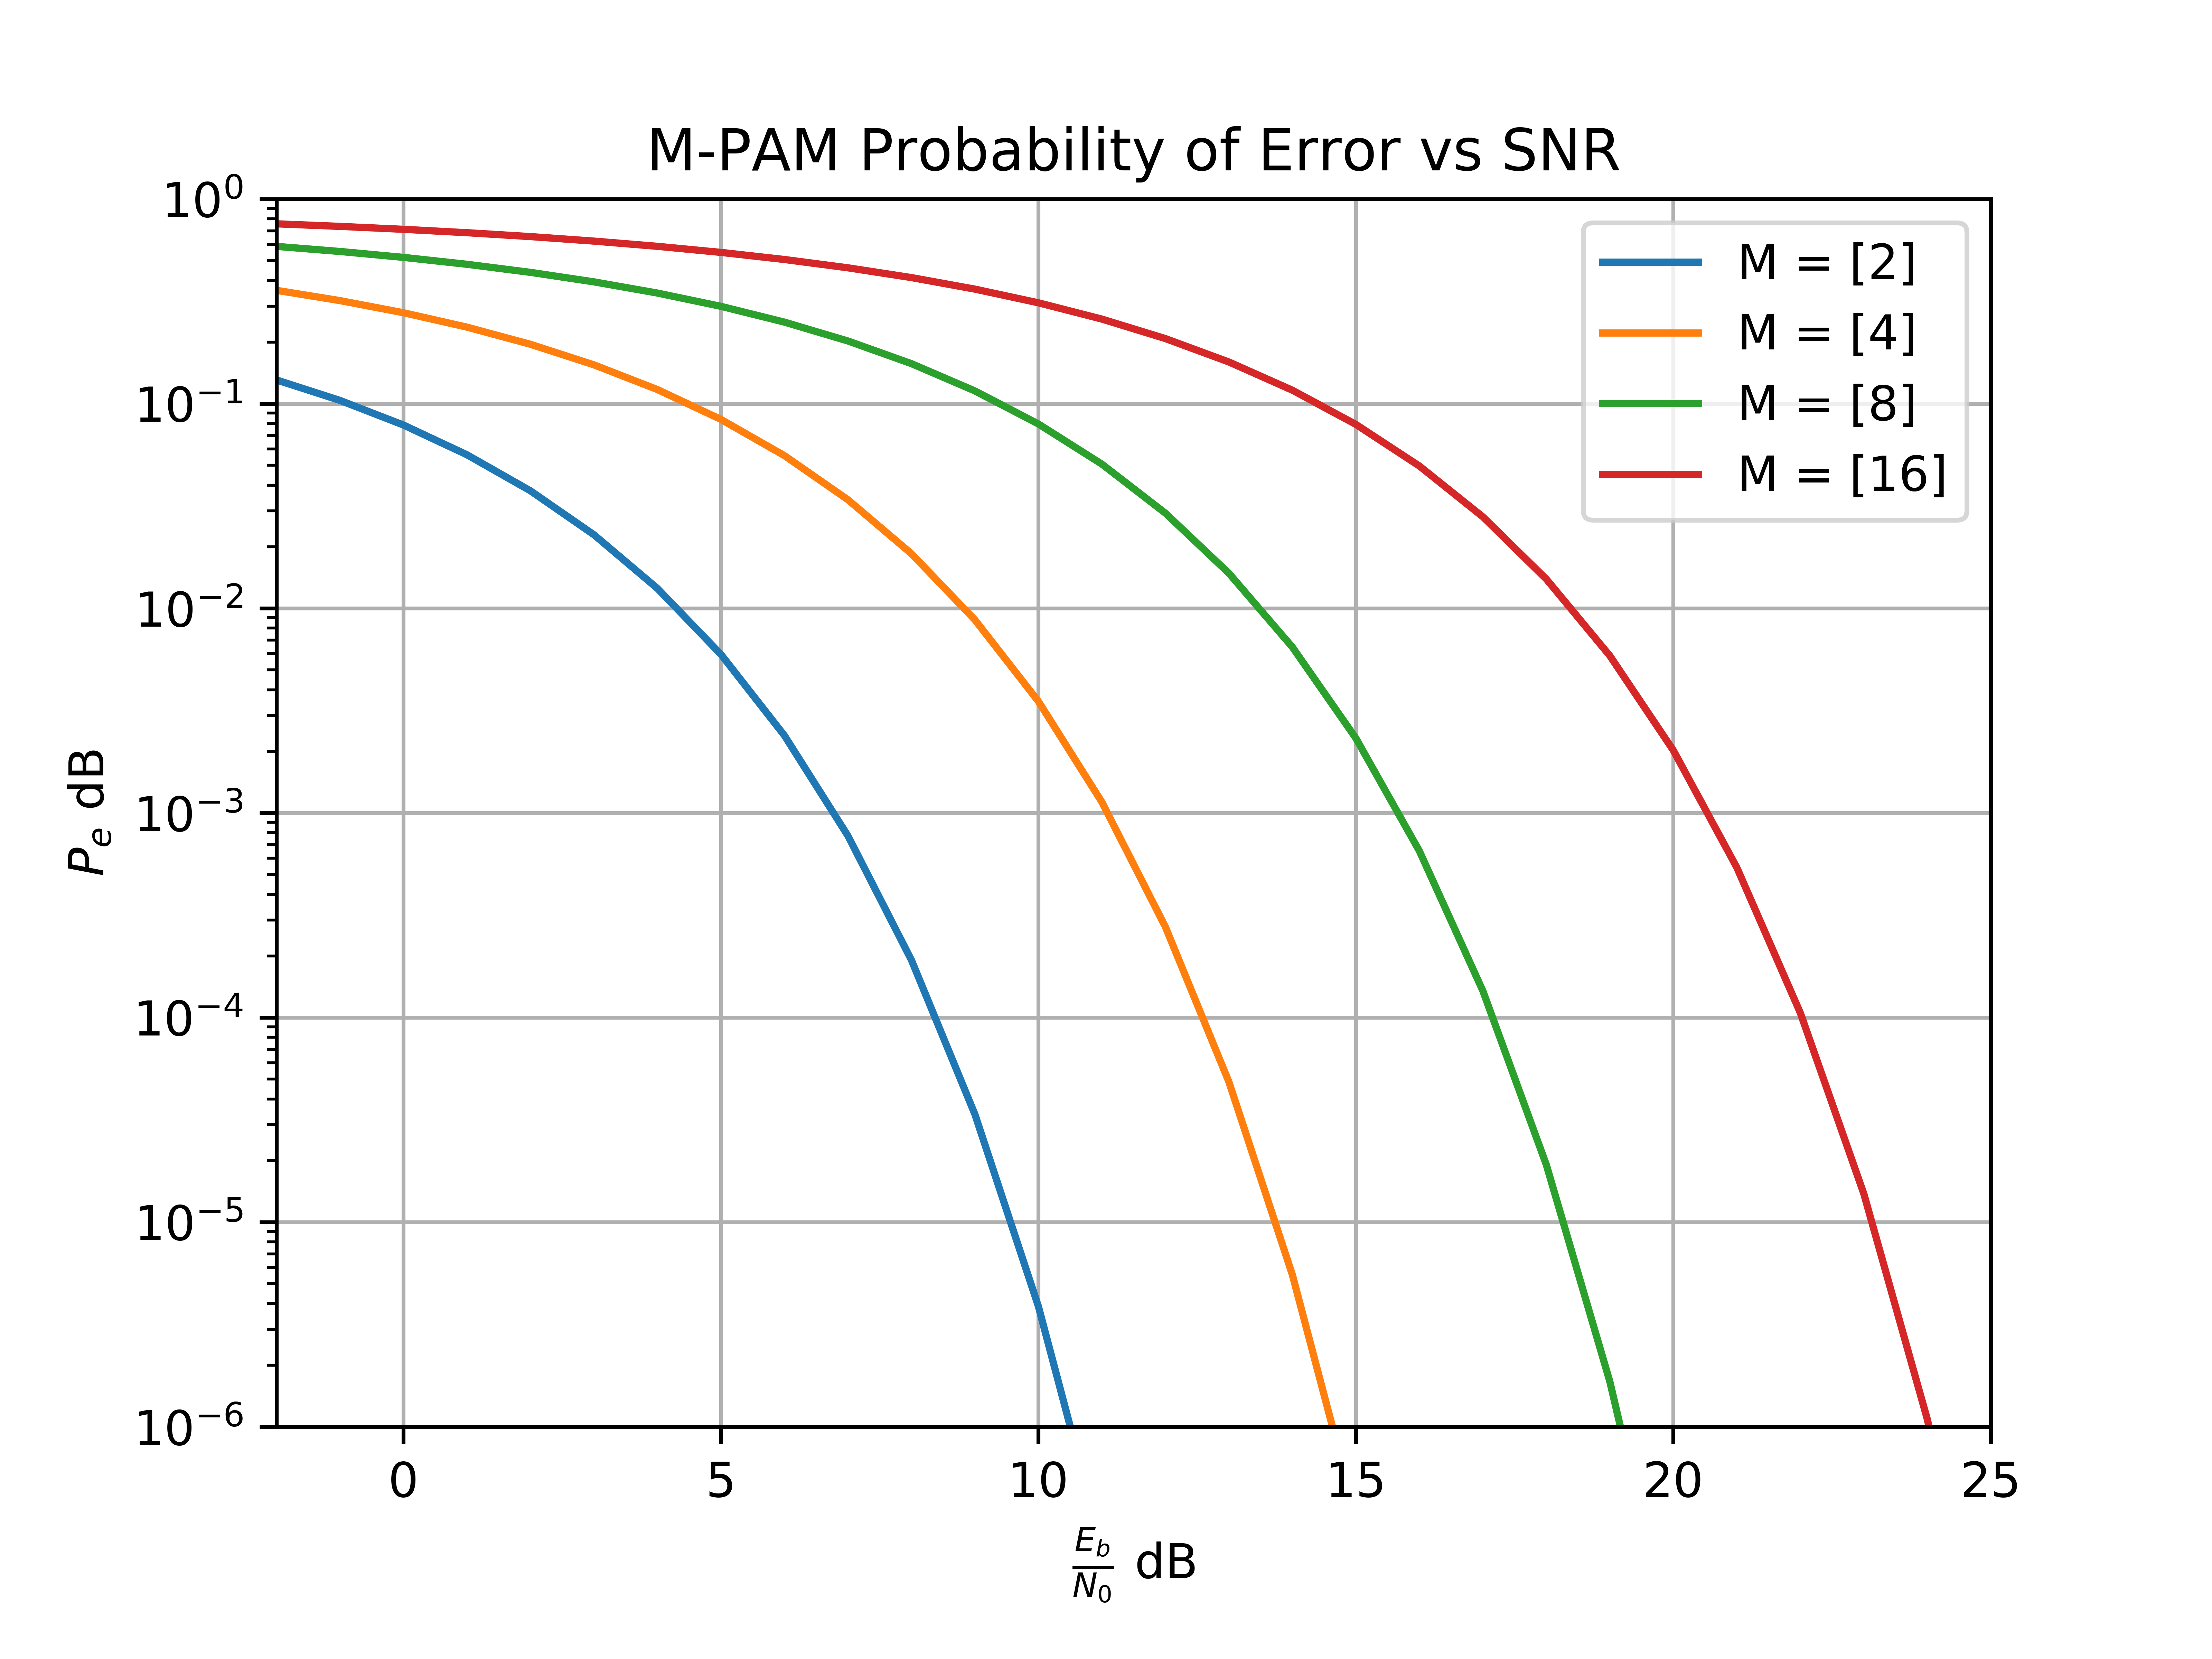
\includegraphics[width=\linewidth]{imagens_ex1/pam.png}\caption{Probabilidade de Erro em função da Razão Sinal-Ruído -- Fonte: O Autor}\label{pamI}
	\end{figure}
	\subsection{Modulação M-QAM}
	Foi utilizada a Equação \eqref{qam} para calcular a SER desta modulação. Com isso, foram plotadas as curvas encontradas em Figura \ref{qamI}.
	\begin{dmath}
	P_e  = 4\left(1-\frac{1}{\sqrt{M}} \right) Q\left( \sqrt{\frac{3\log_2M\,SNR}{M=1}} \right)\left(1-\left(1-\frac{1}{\sqrt{M}}\right) Q\left( \sqrt{\frac{3\log_2M\,SNR}{M=1}} \right) \right)
	\label{qam}
	\end{dmath}
	\begin{figure}[h]\centering
		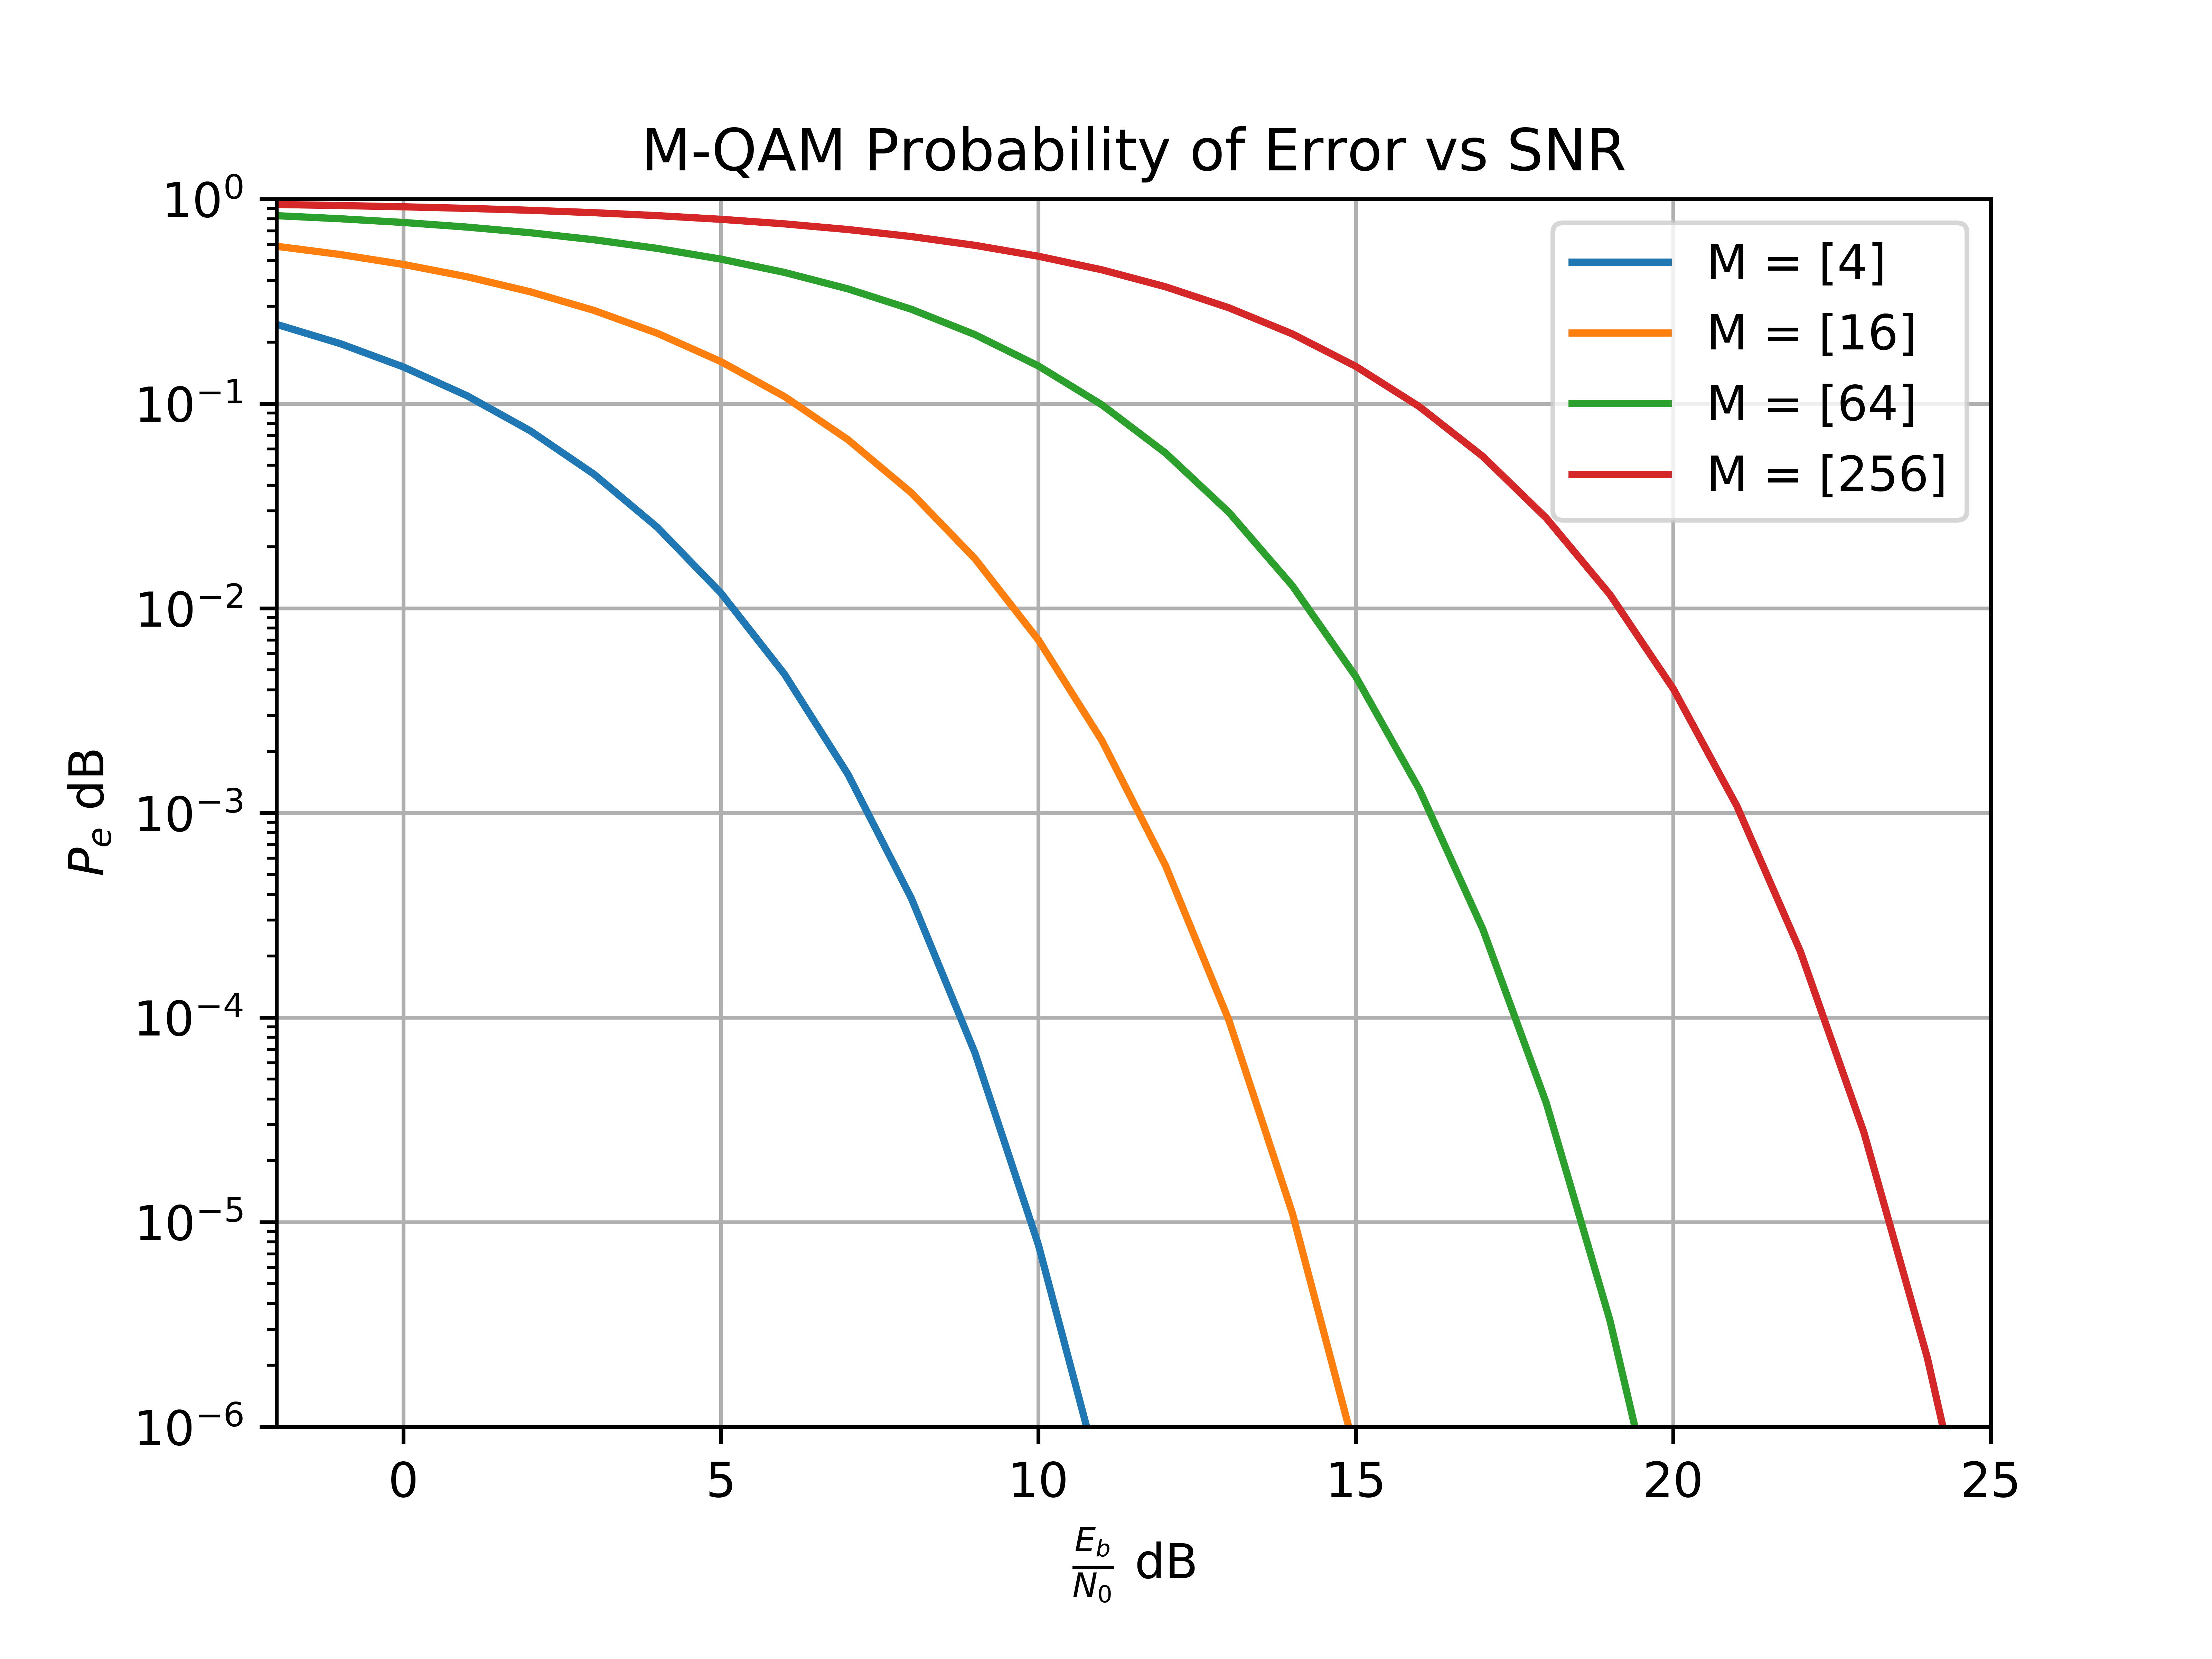
\includegraphics[width=\linewidth]{imagens_ex1/qam.png}\caption{Probabilidade de Erro em função da Razão Sinal-Ruído -- Fonte: O Autor}\label{qamI}
	\end{figure}
	\subsection{Modulação M-PSK}
	Foi utilizada a Equação \eqref{psk} para calcular a SER desta modulação, para $M>4$, para $M=2$ e $M=4$, foram utilizadas respectivamente as Equações \eqref{bpskE} e \eqref{psk4E}. Com isso, foram plotadas as curvas encontradas em Figura \ref{pskI}.
	\begin{equation}
	P_e = Q(\sqrt{2*SNR})\label{bpskE}
	\end{equation}
	\begin{equation}
	P_e = 1-(1-Q(\sqrt{2*SNR}))^2\label{psk4E}
	\end{equation}
	\begin{dmath}
		P_e  = 2 Q\left( \sqrt{2 \log_2M \sin^2(\pi/M)*SNR}\right) 
		\label{psk}
	\end{dmath}
	\begin{figure}[h]\centering
		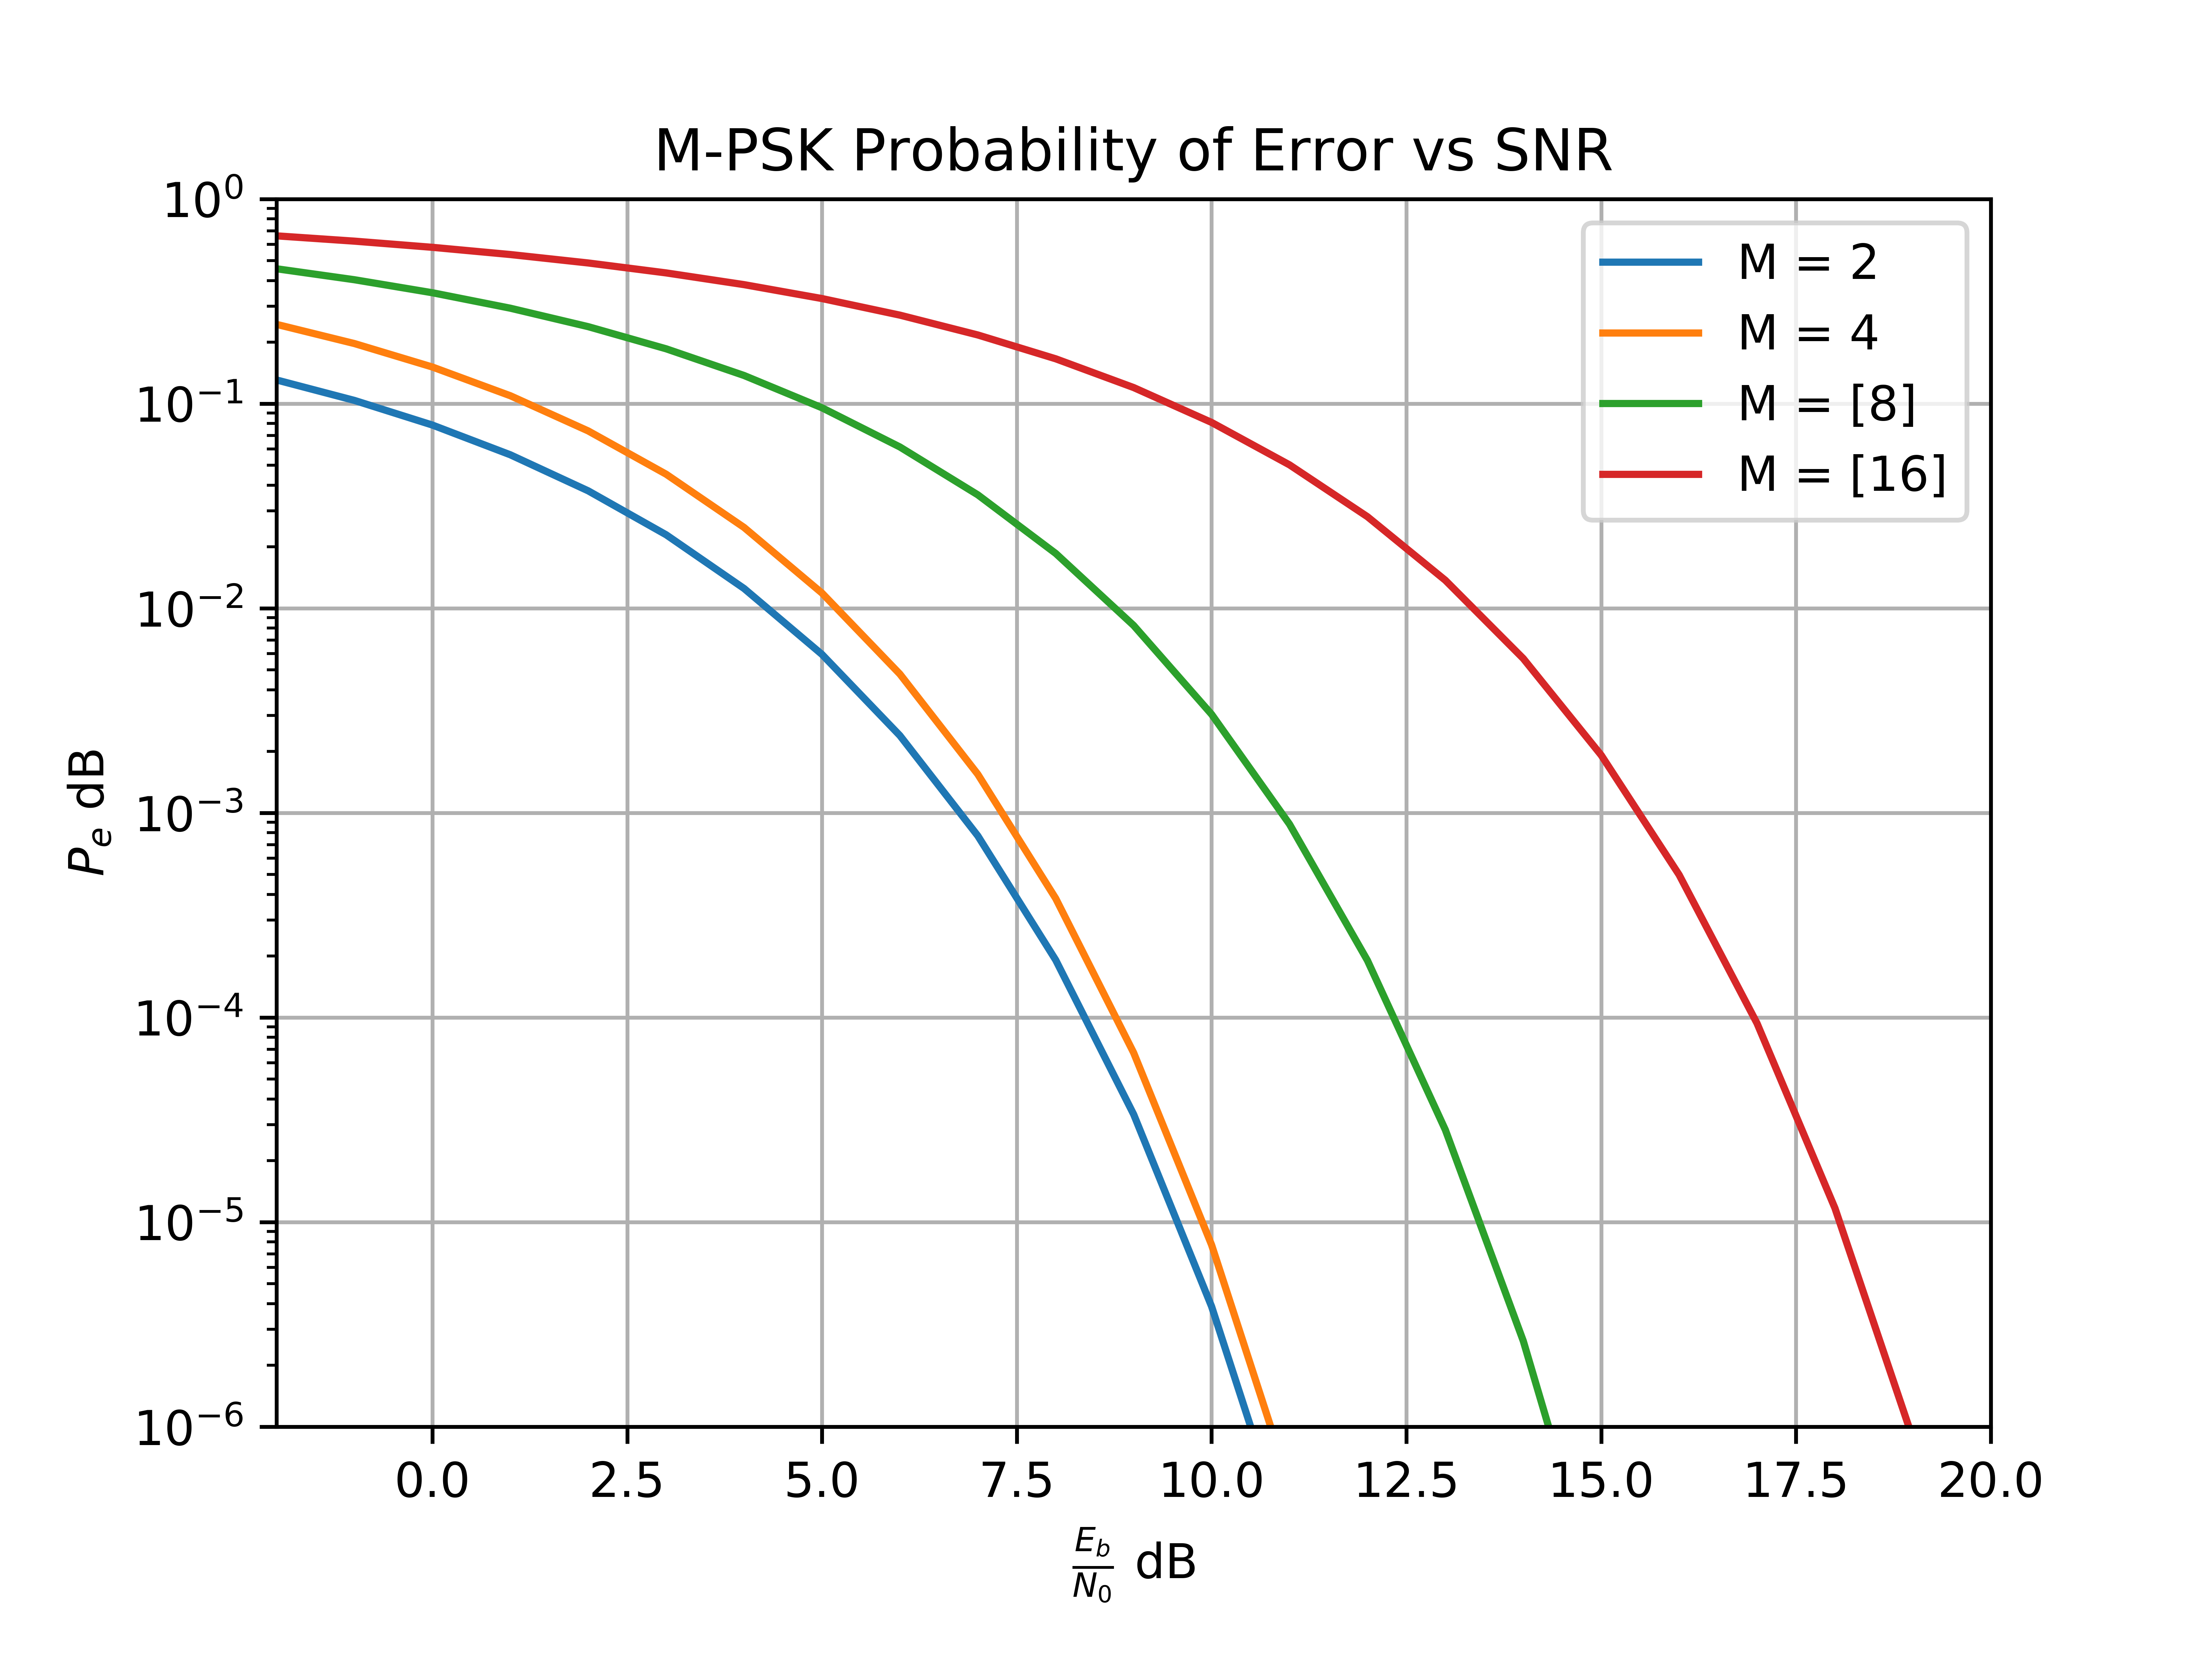
\includegraphics[width=\linewidth]{imagens_ex1/psk.png}\caption{Probabilidade de Erro em função da Razão Sinal-Ruído -- Fonte: O Autor}\label{pskI}
	\end{figure}
	\subsection{Modulação M-FSK}
	Foi utilizada a Equação \eqref{fsk} para calcular a SER desta modulação. Com isso, foram plotadas as curvas encontradas em Figura \ref{fskI}.
	\begin{dmath}
		P_e  = \frac{M-1}{2}erfc\left(\sqrt{\frac{SNR*\log_2(M)}{2}}\right)
		\label{fsk}
	\end{dmath}
	\begin{figure}[h]\centering
		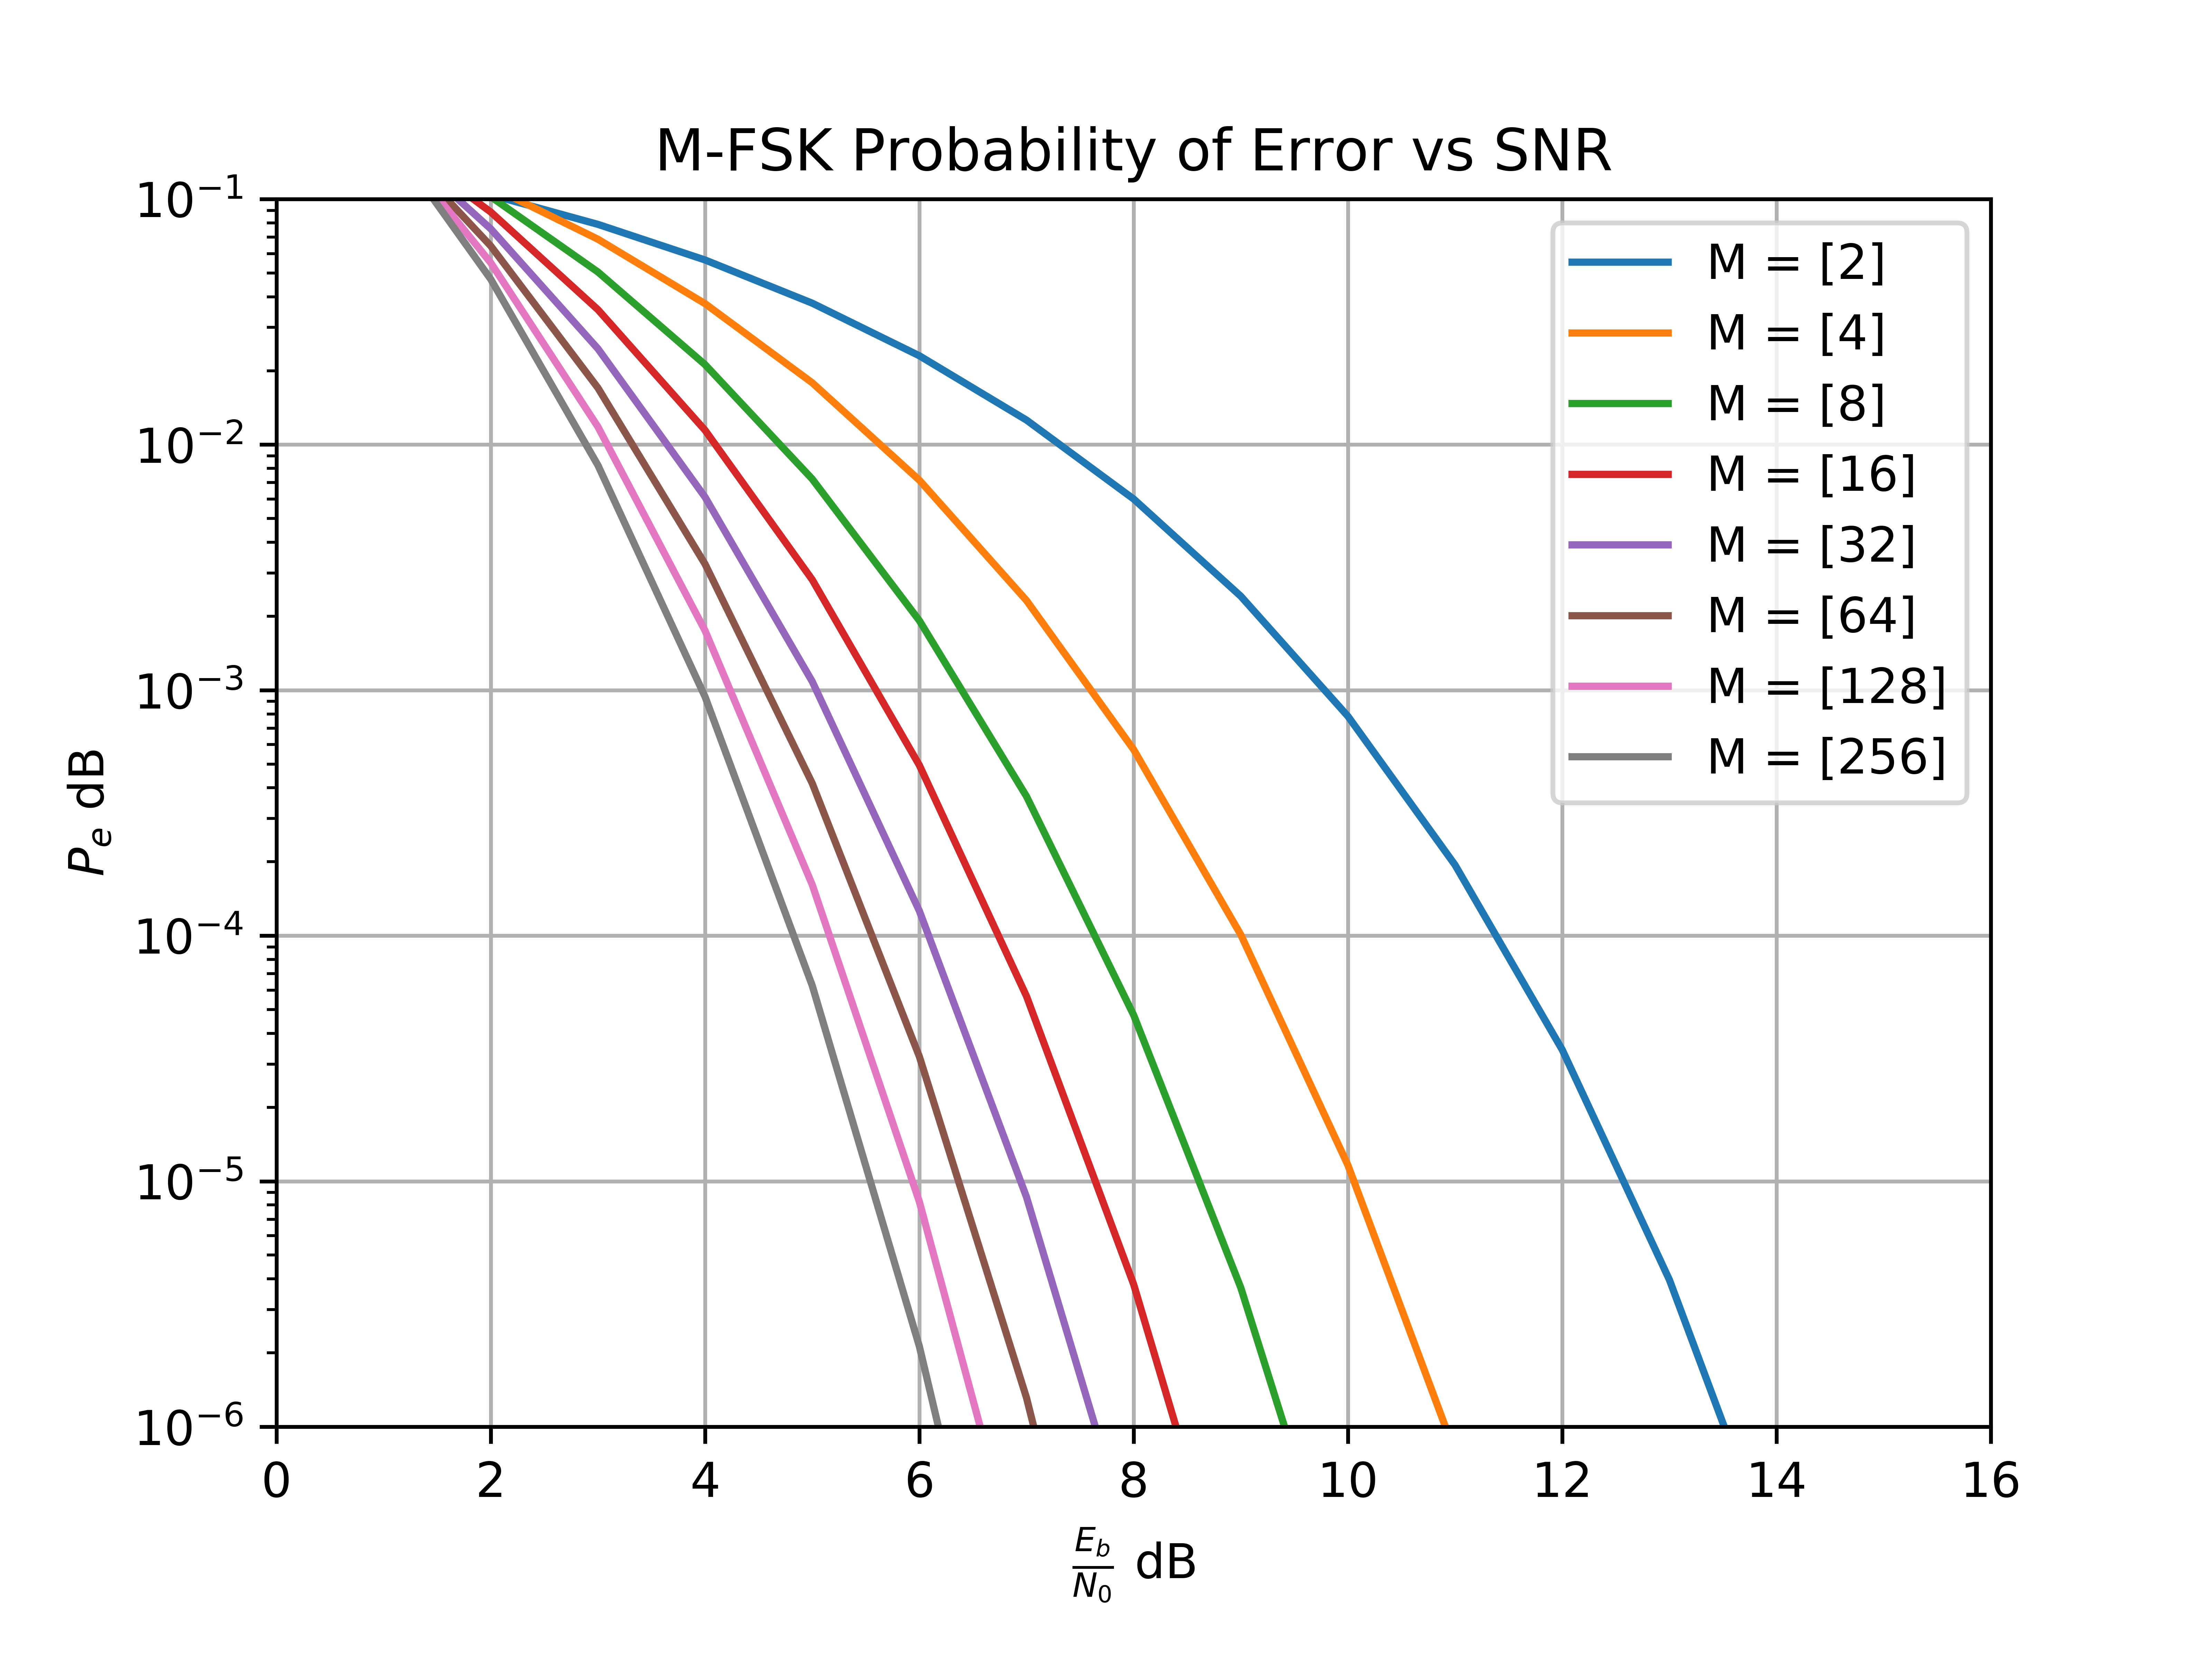
\includegraphics[width=\linewidth]{imagens_ex1/fsk.png}\caption{Probabilidade de Erro em função da Razão Sinal-Ruído -- Fonte: O Autor}\label{fskI}
	\end{figure}
	\section{Exercício 2}
	\todo[inline]{Estime, através de simulação computacional (método de Monte Carlo), a probabilidade de erro de símbolo ($P_e$) em função da razão sinal-ruído por bit ($E_b/N_0$) para as modulações a seguir:}
	\begin{enumerate}
		\item[a$)$] 2-PAM (BPSK)
		\item[b$)$] 4-PAM
		\item[c$)$] 2-QAM (QPSK)
		\item[d$)$] 2-FSK (BFSK)\end{enumerate}	
	Todas as modulações em questão foram feitas em banda-base, a fim de necessitar menos recurso computacional. O código utilizado se encontra no apêndice.
	Todas as modulações seguiram os passos seguintes:
	\begin{enumerate}
		\item Criar array de SNR em dB para a simulação de Monte Carlo.
		\item Para cada SNR, foi feita uma simulação de Monte Carlo, até que se atendesse o requisito de mínima quantidade de erros, ou estourasse o número máximo de repetições (a fim de evitar loop infinito).
		\item Na simulação de Monte Carlo, foi criado para cada geração, um array de binário, simbolizando a mensagem a ser transmitida, um ruído gaussiano representando o canal AWGN. Foi modulada a mensagem, adicionado o ruído, e então demodulado o sinal.
		\item Foi comparado então o sinal demodulado com o original, e contabilizados os erros, até o requisito de número de erros ser atendido.
		\item Por último retorna o valor da SNR e da BER/SER, para ser exportado em um arquivo CSV (Utilizado para plotar depois com a biblioteca PGFPLOTS).
	\end{enumerate}
	\subsection{2-PAM (BPSK)}
	Na modulação BPSK, obteve-se a curva de probabilidade de erro representada na Figura \ref{bpskMC}.
	\begin{figure}[h]\centering
		\begin{tikzpicture}[xscale=0.9,yscale=0.9]
		\begin{semilogyaxis}[
		xlabel=$E_b/N_0$,ylabel=$P_b$ Error Probability,title=\bfseries Probabilidade de Erro de Bit -- Modulação BPSK,
		grid=both,grid style={line width=.2pt, draw=gray},
		major grid style={line width=.1pt,draw=gray},
		minor tick num=1]
		\addplot[color=blue,mark=*] table{montecarlo/bpsk.csv};
		\end{semilogyaxis}
		\end{tikzpicture}
		\caption{Simulação de Monte Carlo -- Fonte: O Autor}\label{bpskMC}
	\end{figure}
	A Figura \ref{bpskComp} compara com a curva encontrada no Exercício 1.
	\begin{figure}[h]\centering
		\begin{tikzpicture}[xscale=0.9,yscale=0.9]
		\begin{semilogyaxis}[
		xlabel=$E_b/N_0$,ylabel=$P_b$ Error Probability,title=\bfseries Probabilidade de Erro de Bit -- Modulação BPSK,
		grid=both,grid style={line width=.2pt, draw=gray},
		major grid style={line width=.1pt,draw=gray},
		minor tick num=1,legend style={font=\tiny}, ymin=1e-6,ymax=1e-1]
		\addplot[color=blue,mark=*] table{montecarlo/bpsk.csv};
		\addplot[color=red,mark=x] table[x index=0,y index=1]{imagens_ex1/pam_teorico2.csv};
		\legend{Simulação de Monte Carlo,Curva Teórica}
		\end{semilogyaxis}
		\end{tikzpicture}
		\caption{Comparativo Simulação de Monte Carlo vs SER Teórica -- Fonte: O Autor}\label{bpskComp}
	\end{figure}

	\subsection{4-PAM}
	Na modulação 4-PAM, obteve-se a curva de probabilidade de erro representada na Figura \ref{4pamMC}.
	\begin{figure}[h]\centering
		\begin{tikzpicture}[xscale=0.9,yscale=0.9]
		\begin{semilogyaxis}[ymax=2.5,xmin=1.2,
		xlabel=$E_b/N_0$,ylabel=$P_e$ Error Probability,title=\bfseries Probabilidade de Erro de Símbolo -- Modulação 4-PAM,ymin=1e-6,ymax=1e-1,xmin=5,xmax=14,
		grid=both,grid style={line width=.2pt, draw=gray},
		major grid style={line width=.1pt,draw=gray},
		minor tick num=1,legend style={font=\tiny}]
		\addplot[color=blue,mark=*] table{montecarlo/4pam.csv};
		\end{semilogyaxis}
		\end{tikzpicture}
		\caption{Simulação de Monte Carlo -- Fonte: O Autor}\label{4pamMC}
	\end{figure}
	A Figura \ref{4pamComp} compara com a curva encontrada no Exercício 1.
	\begin{figure}[h]\centering
		\begin{tikzpicture}[xscale=0.9,yscale=0.9]
		\begin{semilogyaxis}[ymax=2.5,xmin=1.2,
		xlabel=$E_b/N_0$,ylabel=$P_e$ Error Probability,title=\bfseries Probabilidade de Erro de Símbolo -- Modulação 4-PAM,ymin=1e-6,ymax=1e-1,xmin=5,xmax=14,
		grid=both,grid style={line width=.2pt, draw=gray},
		major grid style={line width=.1pt,draw=gray},
		minor tick num=1,legend style={font=\tiny}]
		\addplot[color=blue,mark=*] table{montecarlo/4pam.csv};
		\addplot[color=red,mark=x] table[x index=0,y index=2]{imagens_ex1/pam_teorico2.csv};
		\legend{Simulação de Monte Carlo,Curva Teórica}
		\end{semilogyaxis}
		\end{tikzpicture}
		\caption{Comparativo Simulação de Monte Carlo vs SER Teórica -- Fonte: O Autor}\label{4pamComp}
	\end{figure}
	\subsection{4-QAM (QPSK)}
	Na modulação QPSK, obteve-se a curva de probabilidade de erro representada na Figura \ref{qpskMC}.
	\begin{figure}[h]\centering
		\begin{tikzpicture}[xscale=0.9,yscale=0.9]
		\begin{semilogyaxis}[
		xlabel=$E_b/N_0$,ylabel=$P_e$ Error Probability,title=\bfseries Probabilidade de Erro de Símbolo -- Modulação QPSK,
		grid=both,grid style={line width=.2pt, draw=gray},
		major grid style={line width=.1pt,draw=gray},
		minor tick num=1]
		\addplot[color=blue,mark=*] table{montecarlo/qpsk.csv};
		\end{semilogyaxis}
		\end{tikzpicture}
		\caption{Simulação de Monte Carlo -- Fonte: O Autor}\label{qpskMC}
	\end{figure}
	A Figura \ref{qpskComp} compara com a curva encontrada no Exercício 1.
	\begin{figure}[h]\centering
		\begin{tikzpicture}[xscale=0.9,yscale=0.9]
		\begin{semilogyaxis}[ymax=2.5,xmin=1.2,
		xlabel=$E_b/N_0$,ylabel=$P_e$ Error Probability,title=\bfseries Probabilidade de Erro de Símbolo -- Modulação 4-QAM,ymin=1e-6,ymax=1e-1,xmin=0,xmax=11,
		grid=both,grid style={line width=.2pt, draw=gray},
		major grid style={line width=.1pt,draw=gray},
		minor tick num=1,legend style={font=\tiny}]
		\addplot[color=blue,mark=*] table{montecarlo/qpsk.csv};
		\addplot[color=red,mark=x] table[x index=0,y index=1]{imagens_ex1/qam_teorico2.csv};
		\legend{Simulação de Monte Carlo,Curva Teórica}
		\end{semilogyaxis}
		\end{tikzpicture}
		\caption{Comparativo Simulação de Monte Carlo vs SER Teórica -- Fonte: O Autor}\label{qpskComp}
	\end{figure}
	\subsection{2-FSK (BFSK)}
		Na modulação BFSK, obteve-se a curva de probabilidade de erro representada na Figura \ref{bfskMC}.
	\begin{figure}[h]\centering
	\begin{tikzpicture}[xscale=.9,yscale=.9]
	\begin{semilogyaxis}[
	xlabel=$E_b/N_0$,ylabel=$P_b$ Error Probability,title=\bfseries Probabilidade de Erro de Bit -- Modulação BFSK,
	grid=both,grid style={line width=.2pt, draw=gray},
	major grid style={line width=.1pt,draw=gray},
	minor tick num=1,ymin=1e-6,ymax=1e-1,xmin=2,xmax=13]
	\addplot[color=blue,mark=*] table{montecarlo/bfsk.csv};
	\end{semilogyaxis}
	\end{tikzpicture}
	\caption{Simulação de Monte Carlo -- Fonte: O Autor}\label{bfskMC}
	\end{figure}
	A Figura \ref{bfskComp} compara com a curva encontrada no Exercício 1.
\begin{figure}[h]\centering
	\begin{tikzpicture}[xscale=0.9,yscale=0.9]
	\begin{semilogyaxis}[xlabel=$E_b/N_0$,ylabel=$P_e$ Error Probability,title=\bfseries Probabilidade de Erro de Símbolo -- Modulação BFSK,ymin=1e-6,ymax=1e-1,xmin=2,xmax=13,
	grid=both,grid style={line width=.2pt, draw=gray},
	major grid style={line width=.1pt,draw=gray},
	minor tick num=1,legend style={font=\tiny}]
	\addplot[color=blue,mark=*] table{montecarlo/bfsk.csv};
	\addplot[color=red,mark=x] table[x index=0,y index=1]{imagens_ex1/fsk_teorico2.csv};
	\legend{Simulação de Monte Carlo,Curva Teórica}
	\end{semilogyaxis}
	\end{tikzpicture}
	\caption{Comparativo Simulação de Monte Carlo vs SER Teórica -- Fonte: O Autor}\label{bfskComp}
\end{figure}




%	\begin{figure}[H]\centering
%		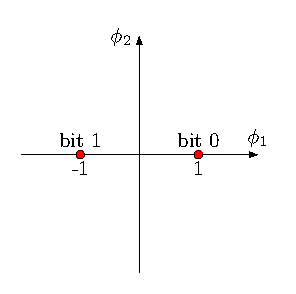
\includegraphics[width=.6\linewidth]{2pam_const}
%		\caption{Constelação Modulação 2-PAM -- Fonte: O Autor}
%	\end{figure}
%	\begin{figure}[H]\centering
%		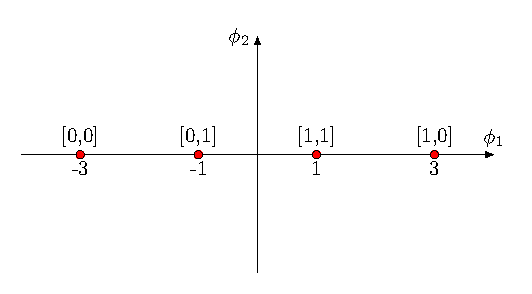
\includegraphics[width=\linewidth]{4pam_const}
%		\caption{Constelação Modulação 4-PAM -- Fonte: O Autor}
%	\end{figure}
%	\begin{figure}[H]\centering
%		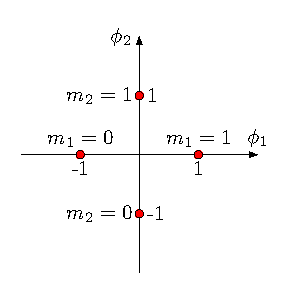
\includegraphics[width=.6\linewidth]{qam_const}
%		\caption{Constelação Modulação 4-QAM -- Fonte: O Autor}
%	\end{figure}
%	\begin{figure}[H]\centering
%		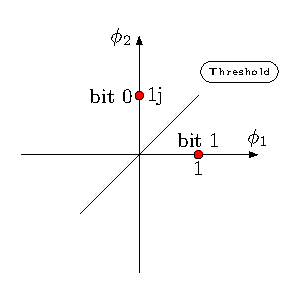
\includegraphics[width=.6\linewidth]{fsk_const}
%		\caption{Constelação Modulação 2-FSK -- Fonte: O Autor}
%	\end{figure}
%	
	\section{Exercício 3}
	\todo[inline]{Repita os itens b-c do problema anterior para estimar a probabilidade de erro de bit ($P_b$) utilizando os seguintes mapeamentos: Mapeamento natural e Mapeamento Gray.}
	
	Seguem nas Figuras \ref{kkkkk} e \ref{llllll} a comparação das modulações utilizando ambos os mapeamentos.
	\begin{figure}[h]
\centering
	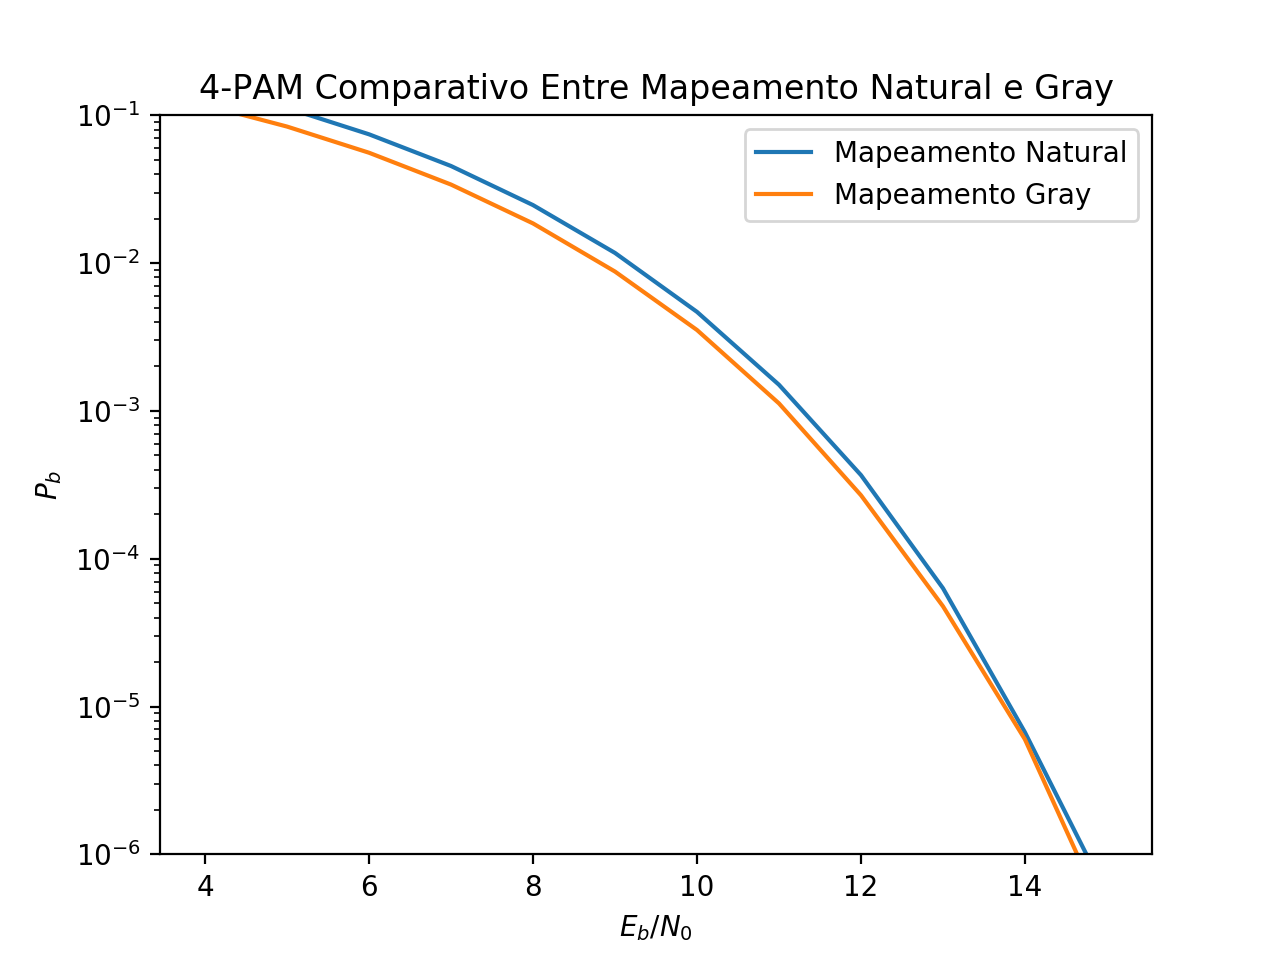
\includegraphics[width=.8\linewidth]{../Exercicio3/PAM3}
	\caption{Modulação 4-PAM Diferença Entre o Mapeamento Natural e Gray}\label{kkkkk}
	\end{figure}
	\begin{figure}[h]
		\centering
		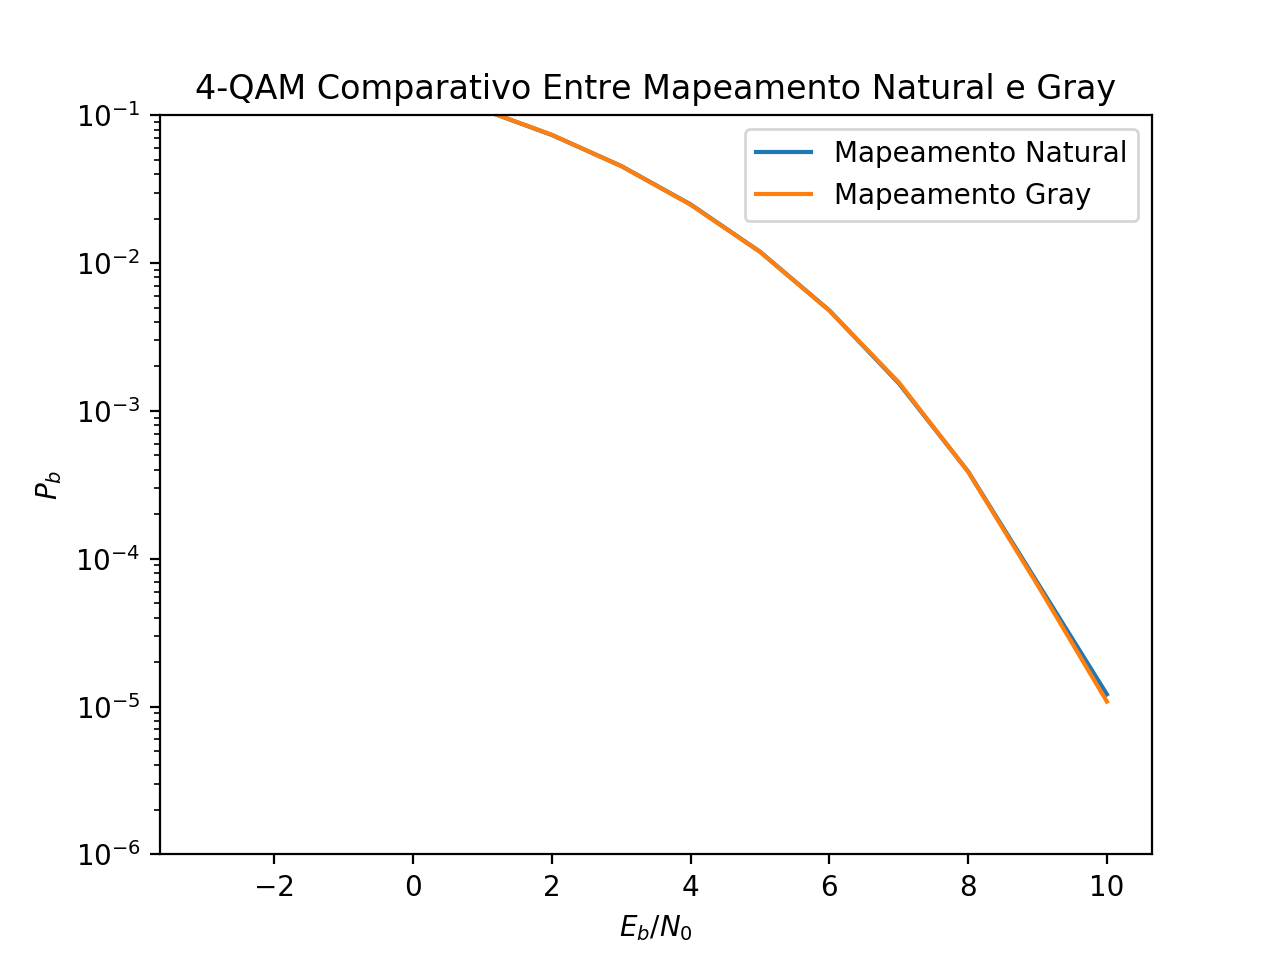
\includegraphics[width=.8\linewidth]{../Exercicio3/QAM3}
		\caption{Modulação 4-QAM Diferença Entre o Mapeamento Natural e Gray}\label{llllll}
	\end{figure}
%	
%	
%%	
%	\bibliographystyle{IEEEtran}
%	\bibliography{bibliografia}
\end{document}